For the geometric distribution the chosen default value is $p=0.001$.
This results in an expected value of 1000 which is the same as for the binomial distribution in the last subsection.
This should make the results more comparable.
Another parameter is the maximum value which was set to $10 \cdot E(X)=10000$.
Theoretically with very low probability the geometric distribution could result in an almost endless loop with bad luck.
To prevent this issue the maximum value was inserted as an upper bound for the random number generator. 
Figure~\ref{fig:geoDistExample} shows that this maximum value does not change the input drastically as no value over 9000 was generated anyway.
The span of all values is way higher than for the binomial distribution, although they have same expected value.
Here the values are not in the interval $[800,1200]$ but rather between 0 and the maximum value. 

\begin{figure}[h]
      \caption{Distribution of a random geometric input}
      \centering
      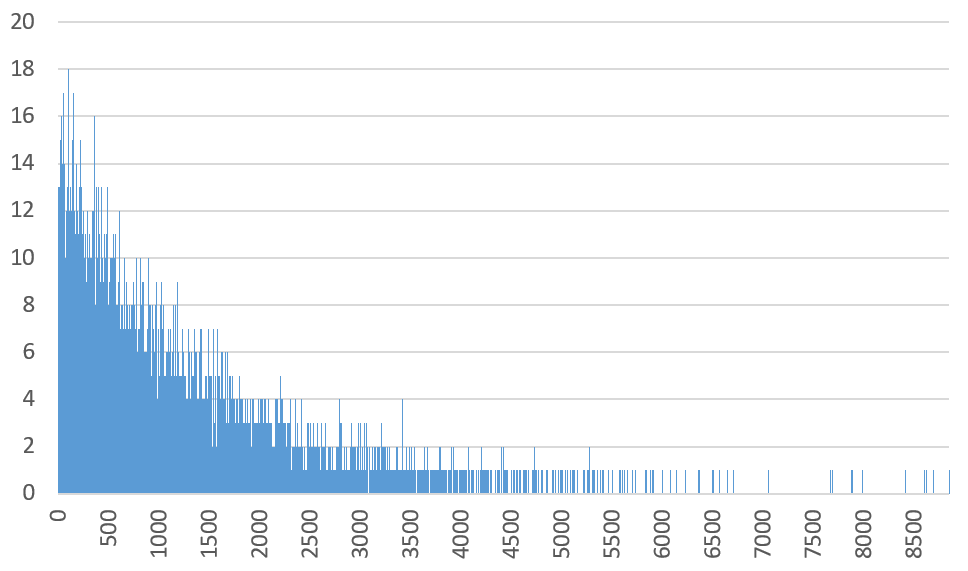
\includegraphics[width=0.7\textwidth]{figures/images/numberGenerator/geometricDistributionForp0_001.png}\label{fig:geoDistExample}
\end{figure}

The geometric distribution does not only have low values close or equal to 1 but also has the most values that are very small.
This should lead to 1-bit flips being effective as the small values can remove the small differences. Because there are so many small values moving only one bit might be better than switching two elements.  